\documentclass[12pt]{article}

\usepackage[margin=1in]{geometry} 
\usepackage{amsmath,amsthm,amssymb}
\usepackage[spanish]{babel}
\usepackage[utf8]{inputenc}
\usepackage{tikz-cd}
\usepackage{amsmath}
\usepackage[shortlabels]{enumitem}
\usepackage{mathtools}
\usepackage{float}
\usepackage{listings}
\usepackage{xcolor}
\usepackage{url}

\graphicspath{{img/}}

\title{SWAP: Práctica 5}
\author{
        Antonio Gámiz Delgado
}

\begin{document}
\maketitle

\section{Preparación inicial}

Primero se debe crear la base de datos en \textit{M1}:

\begin{figure}[H]
\center
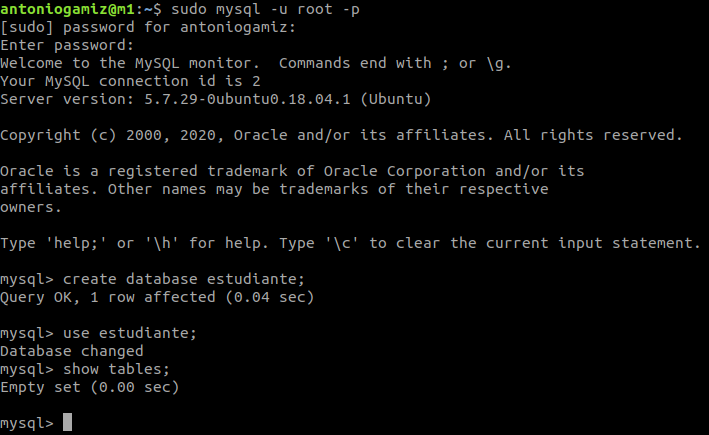
\includegraphics[scale=0.4]{1.png}
\end{figure}

Ahora la tabla que va a ser usada:

\begin{figure}[H]
\center
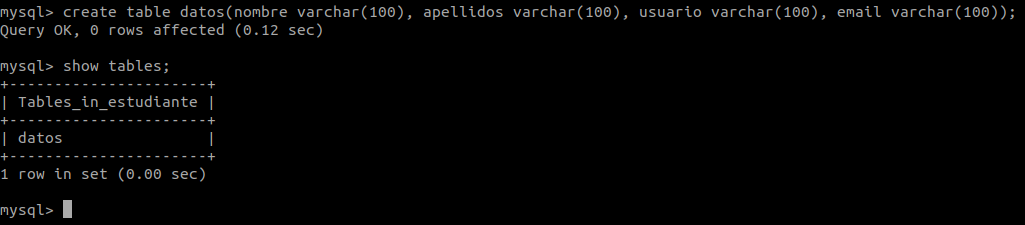
\includegraphics[scale=0.4]{2.png}
\end{figure}

Por último se inserta una tupla de ejemplo:

\begin{figure}[H]
\center
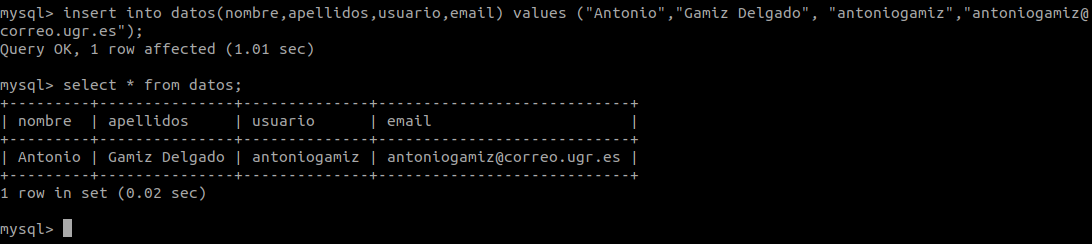
\includegraphics[scale=0.35]{3.png}
\end{figure}

\section{Clonado manual}

Antes de proceder al volcado de los datos, es necesario bloquear el acceso a la base de datos:
\begin{figure}[H]
\center
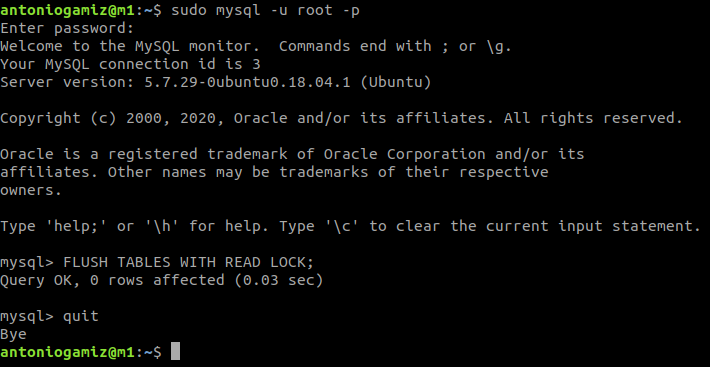
\includegraphics[scale=0.35]{4.png}
\end{figure}
Una vez bloqueado el acceso, se pueden volcar los datos a un fichero:
\begin{figure}[H]
\center
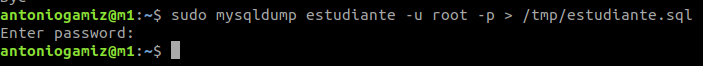
\includegraphics[scale=0.35]{5.png}
\end{figure}
Ya se puede levantar el bloqueo:
\begin{figure}[H]
\center
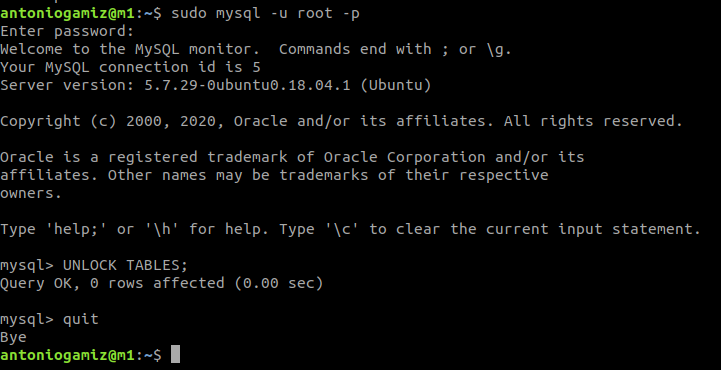
\includegraphics[scale=0.35]{6.png}
\end{figure}
Ahora se clonan los datos a la máquina \textit{M2} usando \textit{M2}:
\begin{figure}[H]
\center
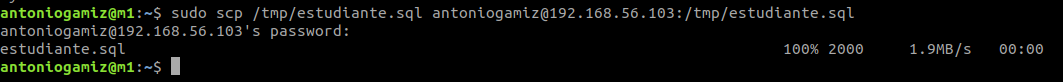
\includegraphics[scale=0.35]{7.png}
\end{figure}
Se crea la base de datos en \textit{M2}:
\begin{figure}[H]
\center
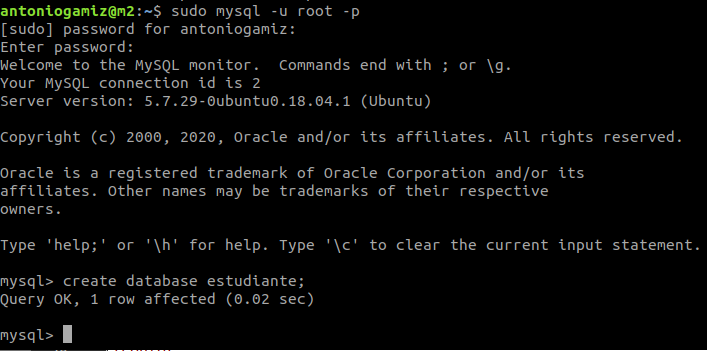
\includegraphics[scale=0.35]{8.png}
\end{figure}
Y se clonan los datos:
\begin{figure}[H]
\center
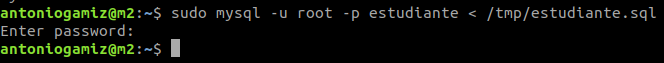
\includegraphics[scale=0.35]{9.png}
\end{figure}

\section{Replicación maestro-esclavo}

Primero se debe modificar el archivo \url{/etc/mysql/mysqld.conf.d/mysqld.cnf} y luego reiniciar \textit{mysql} para aplicar los cambios:
\begin{center}
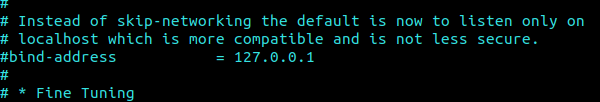
\includegraphics[scale=0.4]{10.png}

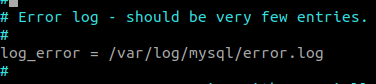
\includegraphics[scale=0.4]{11.png}

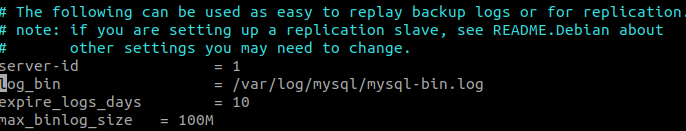
\includegraphics[scale=0.4]{12.png}

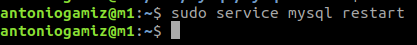
\includegraphics[scale=0.4]{13.png}
\end{center}
Igual en \textit{M2} pero con diferente \textit{server-id}:

\medskip

\begin{center}

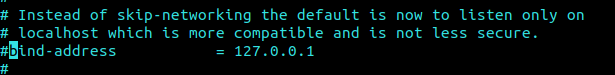
\includegraphics[scale=0.4]{14.png}

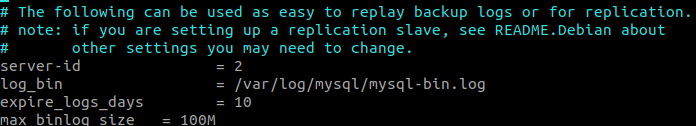
\includegraphics[scale=0.4]{15.png}

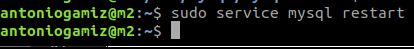
\includegraphics[scale=0.4]{16.png}

\end{center}

Ahora es necesario configurar el maestro en \textit{M1}:
\begin{figure}[H]
\center
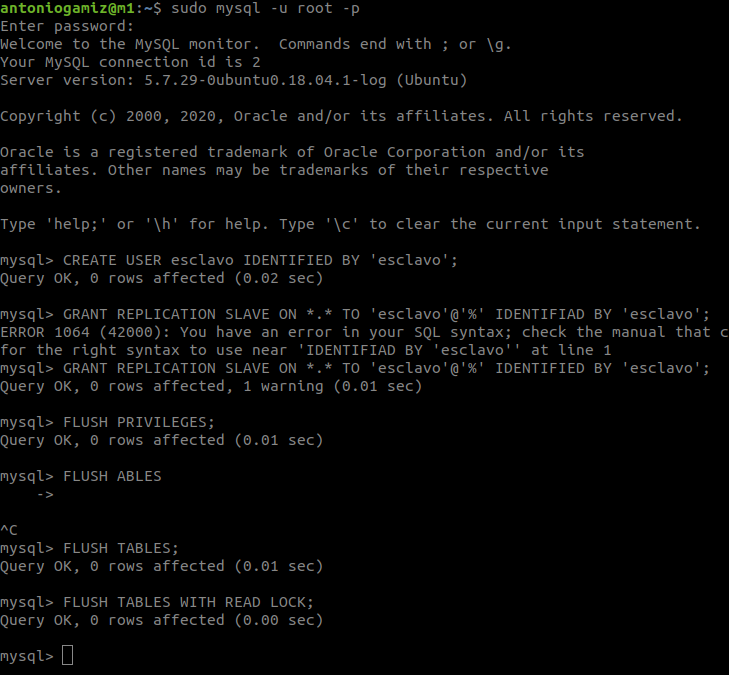
\includegraphics[scale=0.35]{17.png}
\end{figure}
Por si acaso, se comprueba la configuración del maestro:
\begin{figure}[H]
\center
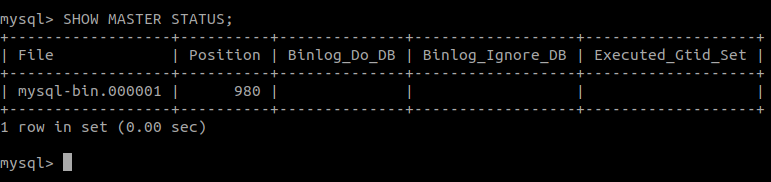
\includegraphics[scale=0.35]{18.png}
\end{figure}
Falta configurar la máquina esclava:
\begin{center}
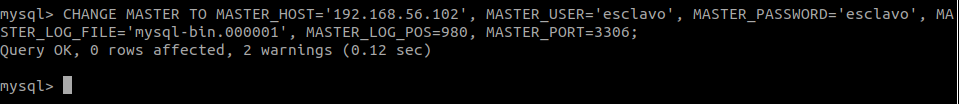
\includegraphics[scale=0.35]{19.png}

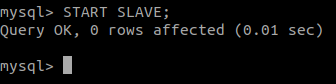
\includegraphics[scale=0.35]{20.png}
\end{center}

Y levantar el bloqueo sobre las tablas de la base de datos de \textit{M1}:
\begin{figure}[H]
\center
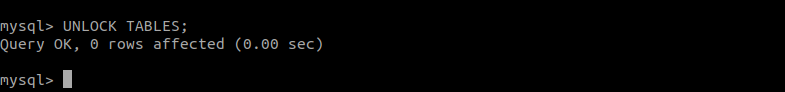
\includegraphics[scale=0.35]{21.png}
\end{figure}

Ya está todo listo. Se puede comprobar que todo funciona correctamente con el siguiente comando:

\begin{figure}[H]
\center
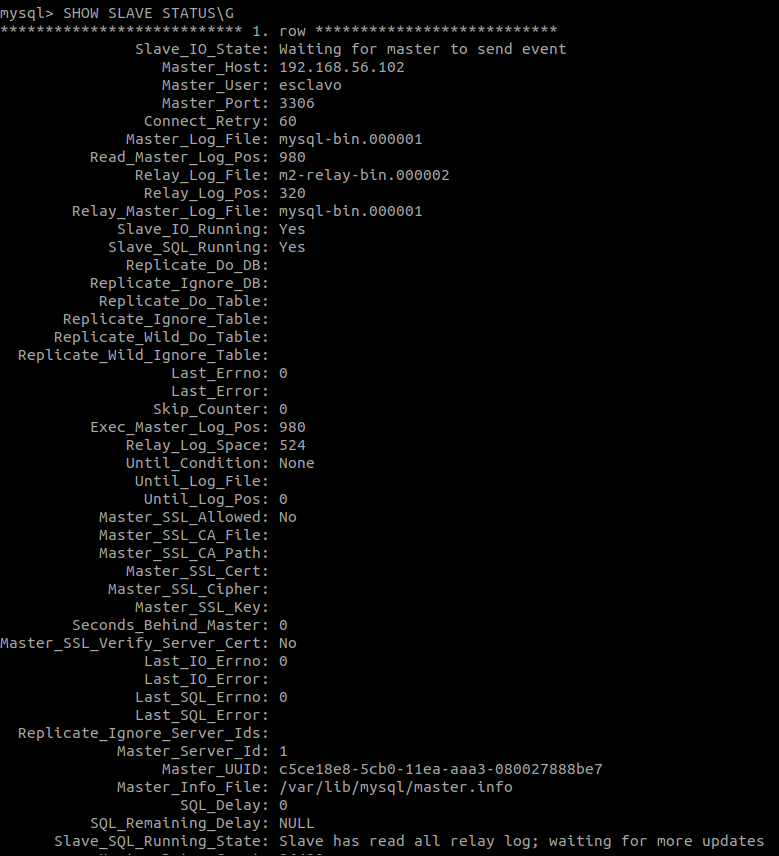
\includegraphics[scale=0.35]{22.png}
\end{figure}

\section{Replicación maestro-maestro}

Básicamente, para conseguir esta configuración lo único que hay que hacer es repetir los mismo pasos del apartado anterior pero cambiando \textit{M1} por \textit{M2} y viceversa. Por esa razón, simplemente añado las capturas:

\begin{center}
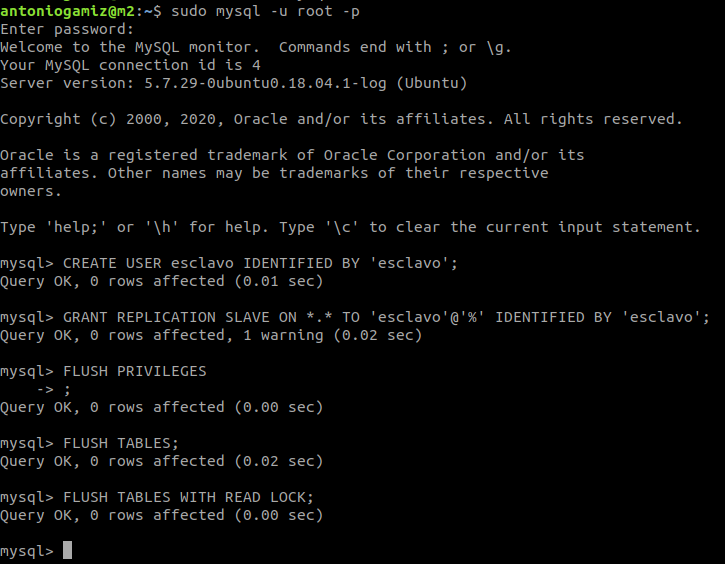
\includegraphics[scale=0.35]{23.png}

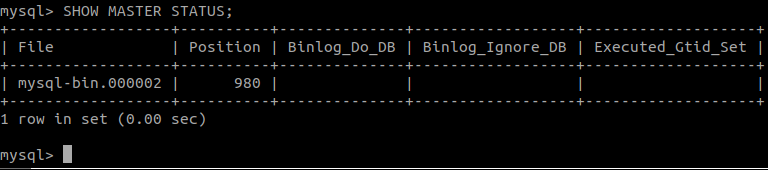
\includegraphics[scale=0.35]{24.png}

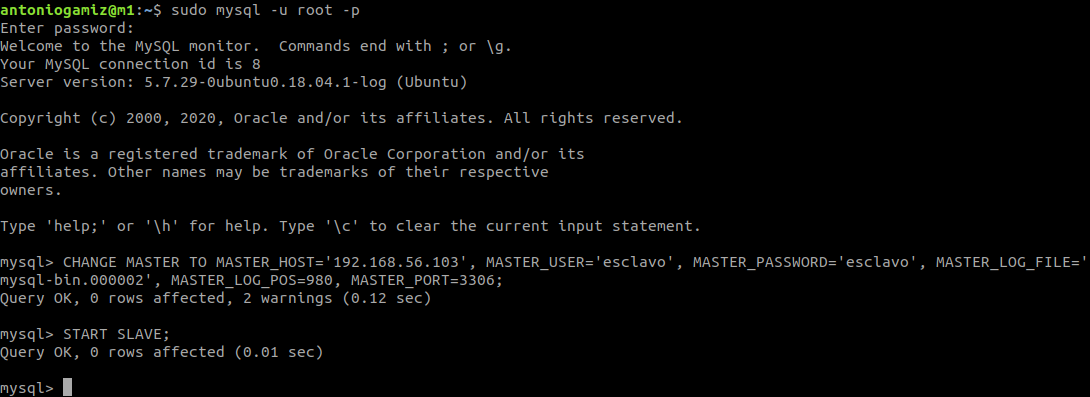
\includegraphics[scale=0.35]{25.png}

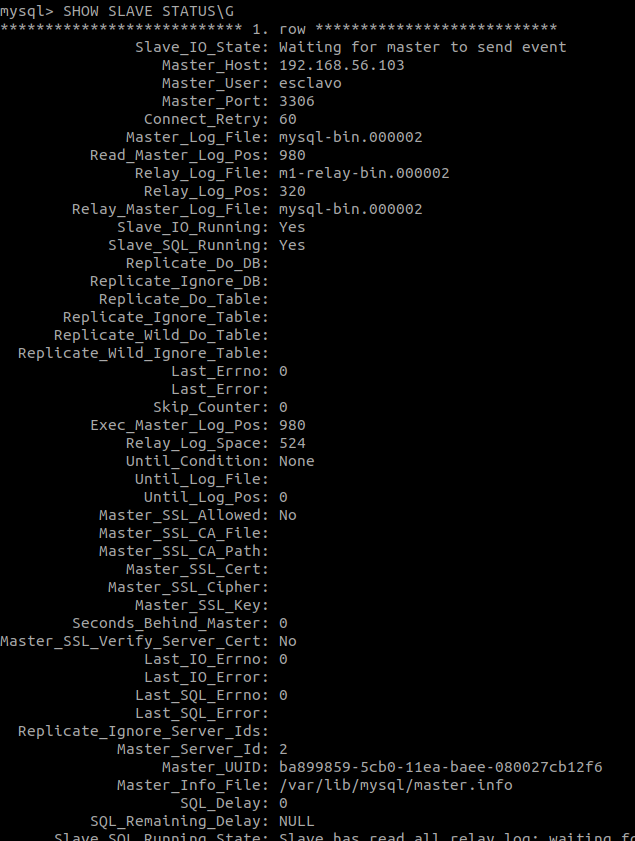
\includegraphics[scale=0.35]{26.png}
\end{center}


\end{document}